\section{问题四的动态电价与信息结构}
\newcommand{\QFourPriceMean}{0.766}
\newcommand{\QFourPriceStd}{0.341}
\newcommand{\QFourPriceMin}{0.0076}
\newcommand{\QFourPriceMax}{1.7936}
\newcommand{\QFourDailyRange}{1.107}
\newcommand{\QFourMaxChange}{0.4996}
\newcommand{\QFourLoadPearson}{0.508}
\newcommand{\QFourLoadSpearman}{0.580}
\newcommand{\QFourNetPearson}{0.260}
\newcommand{\QFourNetSpearman}{0.262}
\newcommand{\QFourValMAE}{0.0382}
\newcommand{\QFourValRMSE}{0.0486}
\newcommand{\QFourOOSMAE}{0.0453}
\newcommand{\QFourOOSRMSE}{0.0624}


\subsection{附件4的数据质量与统计特征}

附件4给出2025年1月1日至12月31日的外网电价，时间分辨率为10 min，单位为元/kWh。按照区间结束时刻展开后，共得到52560条记录，连续覆盖2025年1月1日00:10至2026年1月1日00:00，每日均为144条。数据不存在缺失值、重复时刻、负电价或零电价，与问题二采用的规范运行网格逐点一致。标准化分数绝对值超过3的观测仅作为极值保留，不进行删除或缩尾处理。

\begin{table}[H]
\centering
\small
\caption{附件4动态电价的描述性统计}
\label{tab:q4-price-summary}
\resizebox{\textwidth}{!}{%
\begin{tabular}{lrrrrrrrr}
\toprule
指标 & 均值 & 标准差 & 最小值 & 第一四分位数 & 中位数 & 第三四分位数 & 最大值 & 样本数 \\
\midrule
电价/(元/kWh) & 0.766 & 0.341 & 0.008 & 0.454 & 0.738 & 1.027 & 1.794 & 52560 \\
\bottomrule
\end{tabular}
}
\end{table}


全年平均电价为\QFourPriceMean{}元/kWh，标准差为\QFourPriceStd{}元/kWh，最小值和最大值分别为\QFourPriceMin{}元/kWh和\QFourPriceMax{}元/kWh，表明外网购电成本具有明显的时变性。图\ref{fig:q4-price-annual-monthly}显示，不同月份的电价位置与离散程度均有差异；全年日内价格极差的平均值为\QFourDailyRange{}元/kWh，同一运营日内相邻10 min区间的最大绝对价格变化为\QFourMaxChange{}元/kWh。

\begin{figure}[H]
  \centering
  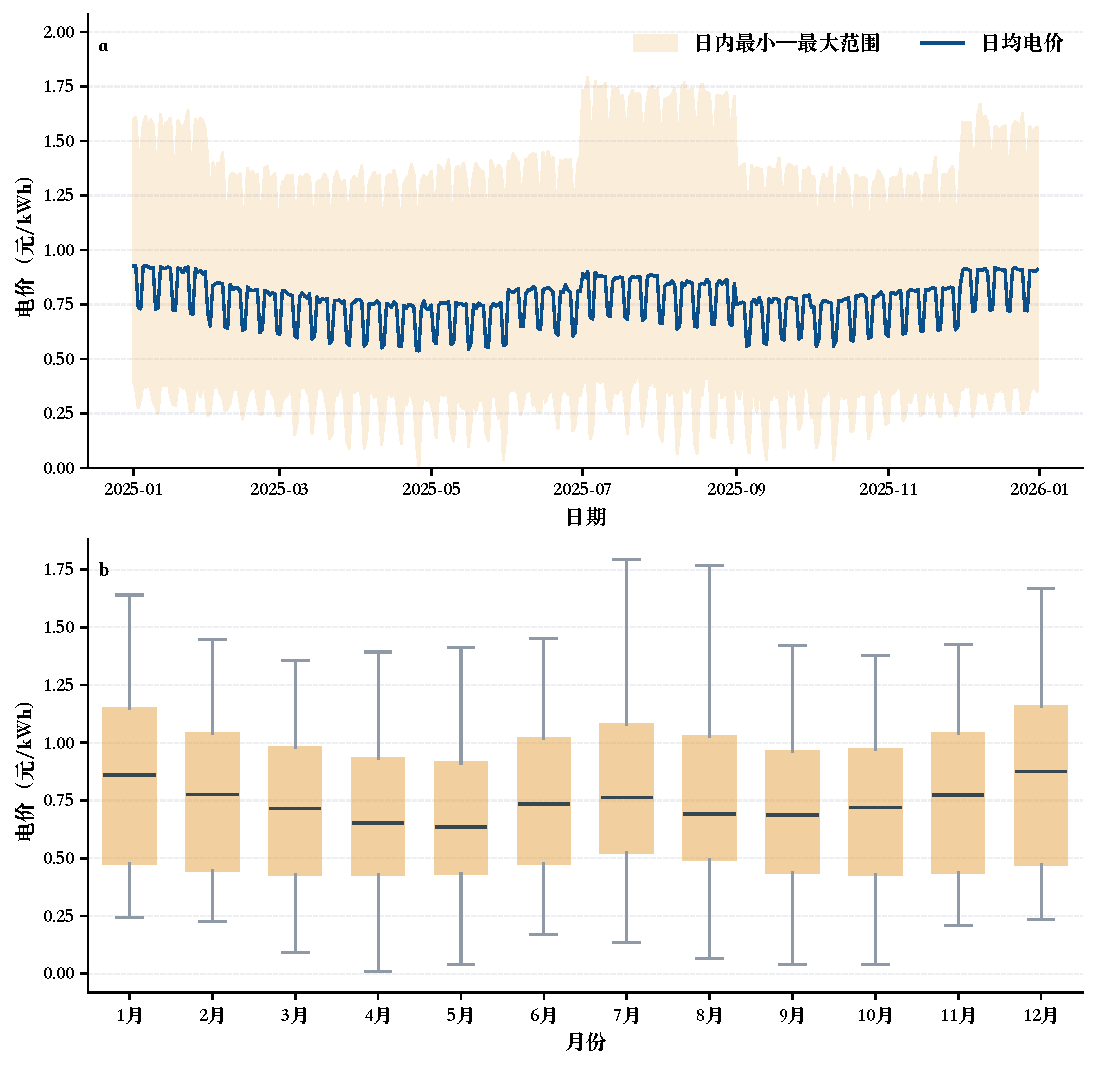
\includegraphics[width=0.88\textwidth]{../results/problem4/figures/fig_p4_price_annual_monthly.pdf}
  \caption{附件4动态电价的全年变化与月度分布}
  \label{fig:q4-price-annual-monthly}
\end{figure}

进一步计算144个日内时段的均值与四分位区间，结果见图\ref{fig:q4-price-intraday}。依据24个小时均价的上下四分位数作数据驱动划分，0:00--4:00及22:00--24:00属于低价小时，8:00--10:00及17:00--21:00属于高价小时。该划分仅刻画样本中的价格结构，不代表预先规定的峰谷电价制度。

\begin{figure}[H]
  \centering
  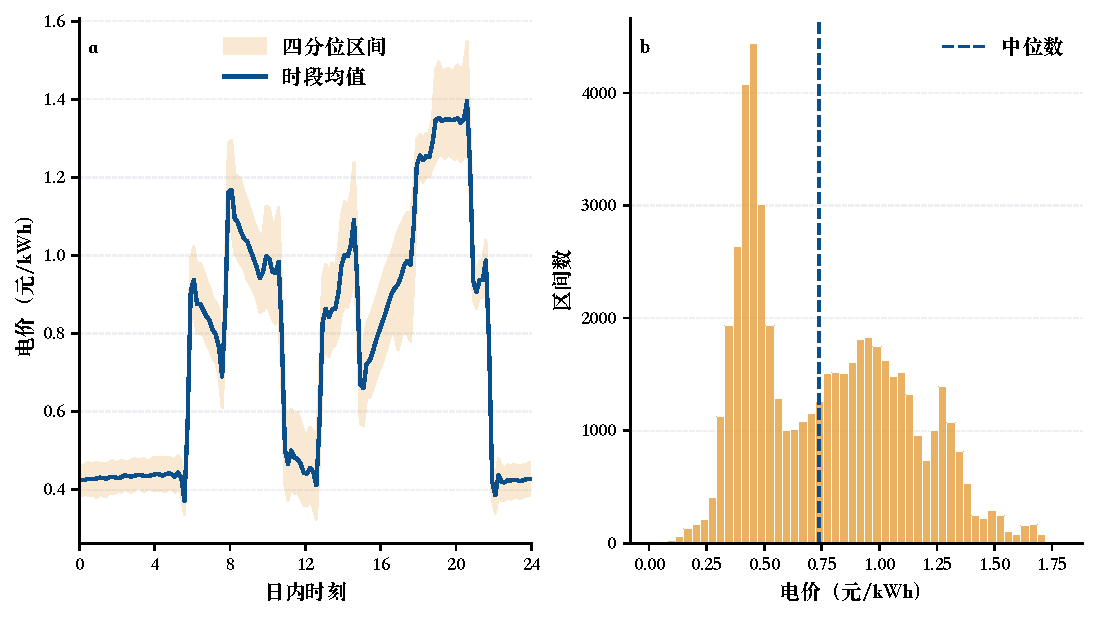
\includegraphics[width=0.92\textwidth]{../results/problem4/figures/fig_p4_price_intraday_distribution.pdf}
  \caption{动态电价的日内轮廓与全年分布}
  \label{fig:q4-price-intraday}
\end{figure}

\subsection{电价与系统运行状态的关联}

为判断价格变化是否与微网用能状态同步，分别计算电价与实际负荷、实际光伏和净负荷的Pearson与Spearman相关系数。净负荷定义为实际负荷减去实际光伏，不对负值截断。

\begin{table}[H]
\centering
\small
\caption{动态电价与系统状态的相关性}
\label{tab:q4-price-correlation}
\begin{tabular}{lrr}
\toprule
系统状态 & Pearson系数 & Spearman系数 \\
\midrule
实际负荷 & 0.508 & 0.580 \\
实际光伏 & 0.028 & 0.189 \\
净负荷 & 0.260 & 0.262 \\
\bottomrule
\end{tabular}
\end{table}


电价与实际负荷的Pearson和Spearman系数分别为\QFourLoadPearson{}和\QFourLoadSpearman{}，呈中等程度正相关；电价与净负荷的两类系数分别为\QFourNetPearson{}和\QFourNetSpearman{}，正相关程度较弱；电价与实际光伏的线性相关性接近于零。上述结果用于描述变量关联，不作因果解释。图\ref{fig:q4-price-system}给出了相关系数和全部52560个区间的电价--净负荷联合分布。

\begin{figure}[H]
  \centering
  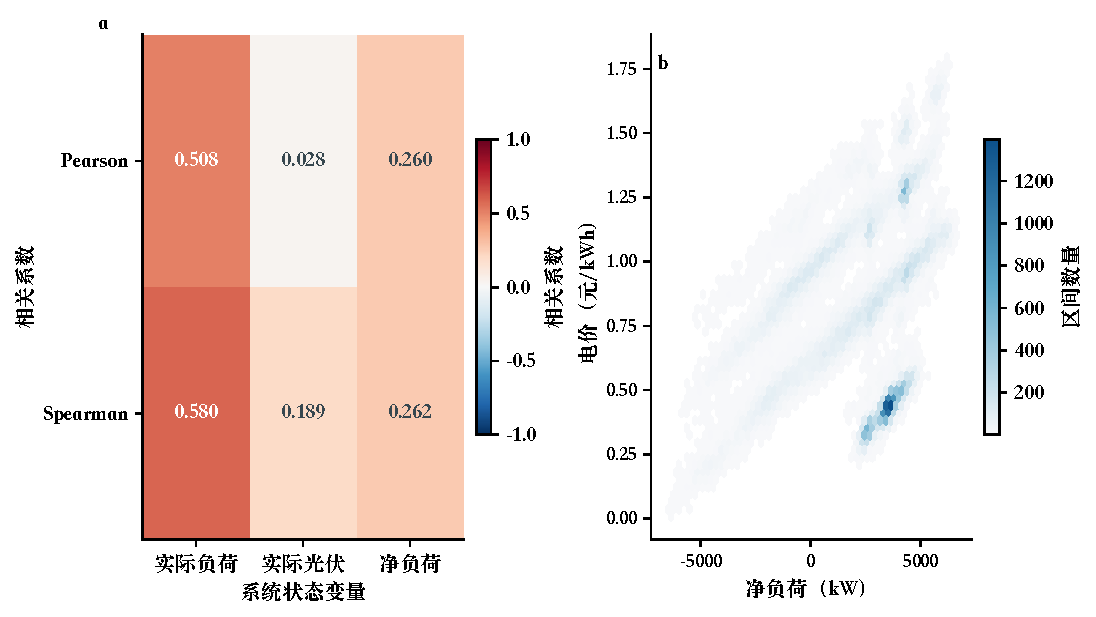
\includegraphics[width=0.94\textwidth]{../results/problem4/figures/fig_p4_price_system_relation.pdf}
  \caption{动态电价与负荷、光伏及净负荷的关联}
  \label{fig:q4-price-system}
\end{figure}

\subsection{未来电价的信息可用性与输入接口}

题面指出外网电价“实时波动”，并要求使用附件4在波动电价下重新计算问题二和问题三，但没有说明每天0:00制定计划时是否能够提前获知全天价格。因此，本文将未来电价可用性判定为不明确，并建立两种互斥的信息模式：完美信息模式直接使用附件4的未来价格，作为理论基准；严格因果模式只允许使用当前时刻之前已经实现的价格和冻结的价格预测。

在因果模式下，比较前一日同刻、前一周同刻、近7日同刻均值和岭回归四种轻量方法。岭回归的输入仅包含历史价格滞后及已知日历周期特征。模型使用1月8日至16日数据拟合，1月17日至30日按RMSE最小、MAE并列判据完成选择，2月1日至12月31日只作冻结样本外评价。最终选择的因果岭回归在验证期的MAE和RMSE分别为\QFourValMAE{}元/kWh和\QFourValRMSE{}元/kWh，在正式评价期分别为\QFourOOSMAE{}元/kWh和\QFourOOSRMSE{}元/kWh。

\begin{figure}[H]
  \centering
  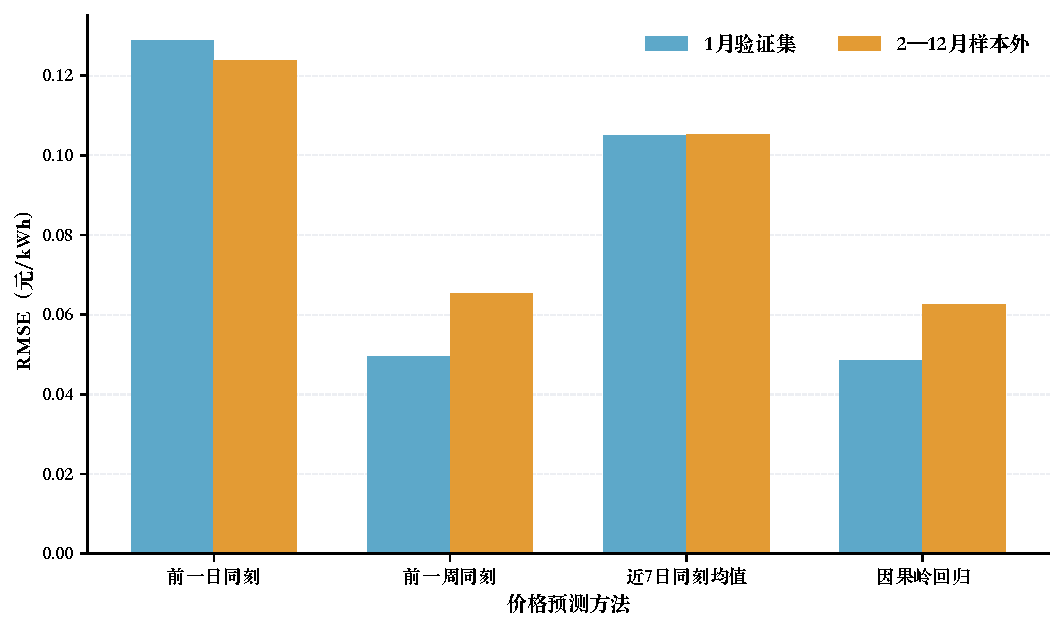
\includegraphics[width=0.82\textwidth]{../results/problem4/figures/fig_p4_price_forecast_comparison.pdf}
  \caption{轻量因果电价预测方法的验证与样本外比较}
  \label{fig:q4-price-forecast}
\end{figure}

价格信息按144个区间组织，并通过已执行区间掩码和未来区间掩码区分历史与待决策时域；在6:00、12:00和18:00，已经执行的区间保持冻结。因果价格路径于日初形成，后续时刻只截取剩余部分，不使用未来实测价格修正。完美信息与因果预测两种模式须分别标注，预测误差的改善不能直接解释为购电成本的降低。
